\chapter{Automatisierte Schmerzbewertung anhand von Schreigeräuschen}
\label{sec:deduction}

In dem vergangenen \autoref{sec:vad} wurden Methoden zur automatisierten Detektion von Schreigeräuschen in Audiosignalen vorgestellt. Dabei wurde erläutert, wie detektierte Schreigeräusche zu Schreieinheiten zusammengefasst werden. Das Ziel dieses Kapitels ist die Vorstellung von Konzepten, um auf Basis der Schreieinheiten die Schmerzbewertung durchzuführen. 

Die Schmerzbewertung des Weinens erfolgt typischerweise nicht aus der Beurteilung einer einzelnen Schreieinheiten, sondern aus der Beurteilung einer Menge mehrerer Schreieinheiten innerhalb eines Beobachtungszeitraumes. Daher ist es zunächst notwendig, erkannte Schreieinheiten so zu gruppieren, das sie gemeinsam einer Schmerzepisode zugeordnet werden können. Diese \emph{Segmentierung} wird in \autoref{sec:segmenting} vorgestellt. Die Möglichkeiten zur Berechnung von Schmerz-Scores anhand objektiv messbarer Eigenschaften des Weinens werden in \autoref{sec:overviewPainRegression} diskutiert.

\section{Zusammenfassung von Schreigeräuschen zu Segmenten}
\label{sec:segmenting}

%Nochemal lesen!
Wie in \autoref{sec:painScores} erläutert wurde, wird die manuelle Schmerzdiagnose bei einem stetigen Monitoring typischerweise umgesetzt, indem Visiten in einer bestimmten Frequenz durchgeführt werden und das Baby bei jeder Visite für einen festgelegten Zeitraum beobachtet wird. Bei jeder Visite werden die Scores für die einzelnen Schmerzindikatoren festgelegt und letztendlich der Schmerzgrad für den jeweiligen Diagnosezeitpunkt bestimmt. So empfiehlt die Schmerz-Scale PAT, das Baby alle 30 Minuten zu überprüfen und jeweils für 15 bis 30 Sekunden zu beobachten. Einige Schmerz-Scales geben keine Empfehlungen für die Beobachtungshäufigkeit und den Beobachtungszeitraum. 

Auch bei einer kontinuierlichen Überwachung durch ein automatisiertes System stellt sich die Frage, zu welchen Zeitpunkten Schmerz-Scores berechnet werden, und welcher beobachtete Zeitraum (\glqq Fenstergröße\grqq ) die Basis der jeweiligen Schmerzbewertung bildet. Es werden zwei Strategien vorgeschlagen:
\begin{enumerate}
\item \textbf{Schmerzdiagnose mit statischen Fenstergrößen: } Es werden feste Werte für die Diagnosefrequenz und den Beobachtungszeitraum festgelegt, ähnlich wie bei der manuellen Schmerzdiagnostik mit Schmerz-Scales. Um die Vorteile eines automatisierten und kontinuierlichen Systems zu nutzen, ist es sinnvoll, die Diagnosefrequenz mit einer weitaus größeren Häufigkeit festzulegen, als es bei der manuellen Überwachung üblich ist. So könnte man beispielsweise alle 2 Sekunden einen Score auf Basis der Informationen der letzten 5 Minuten berechnen. (Diagnosefrequenz $ = \SI{2}{\second}$, Fenstergröße = Beobachtungszeitraum = \SI{5}{\minute}). Diese Strategie ähnelt der, die in dem von Cohen et al. \cite{cohenCry} entwickelten System zur kontinuierlichen Überwachung Neugeborener implementiert wurde (siehe Literaturüberblick in \autoref{sec:system_literature})
\item \textbf{Schmerzdiagnose mit dynamischen Fenstergrößen: } Es wird keine Diagnosefrequenz und kein fester Beobachtungszeitraum festgelegt. Eine Diagnose ruht, solange das Baby keinerlei Anzeichen von Schmerz zeigt. Eine Diagnose wird dann gestartet, sobald das Baby beginnt, potentielle Anzeichen von Schmerz zu zeigen. Wenn das Baby wieder aufhört, potentielle Anzeichen von Schmerz zu zeigen, wird der Schmerz-Score berechnet und die Diagnose beendet. Im Idealfall entspricht ein Diagnosezeitraum einer Schmerzepisode.
\end{enumerate}

Es wurde sich in dieser Arbeit für die zweite Strategie entschieden. Die Begründung ist, dass von den in \autoref{tab:painscores} vorgestellten Schmerz-Scales einige die \emph{Länge des Weinens} als Eigenschaft zur Bestimmung der Schmerzstärke verwenden und somit die Länge der Schmerzepisode selber ein wichtiges Kriterium darstellen kann. Die Verwendung von festen Fensterlängen würde die Bestimmung der genauen Anfangs- und Endzeitpunkte von Schmerzepisoden erschweren.  

Die Berechnung des Schmerz-Score wird zunächst auf das Scoring des Schmerzindikators \emph{Weinen} auf Basis der akustischen Informationen des Audiosignals beschränkt. Unter dieser Einschränkung entspricht ein \glqq potentielles Anzeichen von Schmerz\grqq{} dem \emph{prinzipiellen Vorhandensein von Weingeräuschen}. Aus der Abwesenheit von Weingeräuschen wird zumindest in Bezug auf diesen Schmerzindikator die Abwesenheit von Schmerz geschlossen. Die Ansicht stützt sich auf die Bewertung des Weinens der in \autoref{tab:painscores} vorgestellten Schmerz-Scales, bei denen der überwiegende Teil einen Score von 0 für \glqq kein Weinen\grqq{} vergibt.

%Es ist nicht sinnvoll, dieses Prinzip der Schmerzdiagnose zu festgelegten Visiteintervallen für ein automatisiertes und kontinuierliches System zu übernehmen, da es den Vorteil der Kontinuierlichkeit eliminieren würde.
%Die Frage ist somit, wie eine medizinische Fachkraft das Aufkommen von Schmerz registrieren und den Anfangszeitpunkt der jeweiligen Schmerzdiagnose festlegen würde, würde es das entsprechende Baby kontinuierlich überwachen. Dabei muss bedacht werden, dass eine solche medizinische Fachkraft, so wie das in dieser Arbeit entworfene Systemkonzept, nur die akustischen Informationen zur Verfügung hätte. Die nächst liegende Antwort ist, die Schmerzdiagnose genau dann zu starten, wenn das Baby anfängt, zu weinen. So lange das Baby nicht weint, kann zumindest in Bezug auf diesen Schmerzindikator davon ausgegangen werden, dass kein Schmerz vorliegt (siehe Kapitel \ref{sec:medicalFoundations}).

%Die nächste Frage ist, zu welchem Zeitpunkt die Schmerzdiagnose für die jeweilige Schmerzepisode wieder beendet und ein Schmerz-Score festlegt wird. Da einige Schmerz-Scales aus Tabelle \ref{tab:painscores} Beobachtungszeiträume vorgeben, kann argumentiert werden, dass ein Schmerz-Score direkt nach Beendigung des jeweils angegebenen Beobachtungszeitraums festgelegt werden kann, auch, wenn das Baby weiterhin schreit. Problematisch wären in diesem Fall die Schmerz-Scales, die keine Beobachtungszeiträume vorgeben. Fraglich ist weiterhin, ob eine Vorzeitige Beendigung der Schmerzdiagnose überhaupt sinnvoll ist, wenn ein automatisiertes System zur ständigen Überwachung genau eines Babys vorgesehen ist. Was wäre also der späteste, sinnvolle Zeitpunkt, um nach dem Beginn einer Schmerzepisode einen Schmerz-Score festzulegen und die Diagnose zu beenden? Die nächst liegende Antwort ist: Dann, wenn das Baby wieder aufhört, zu weinen.

Auf Basis dieser Überlegungen wurde das folgende Vorgehen zur kontinuierlichen Segmentierung des Audiosignals entwickelt. Schreieinheiten, die zu einer Schmerzepisode gehören, sollen zu einem \emph{Schrei-Segment} gruppiert werden. So lange das Baby keine Äußerungen von sich gibt, weil es beispielsweise schläft, wird keine Schreieinheit in dem Audiosignal festgestellt, womit für diesen Zeitbereich auch kein Segment existiert. Fängt das Baby an, einen Laut von sich zu geben, welcher vom System als Schreieinheit detektiert wird, wird ein neues Segment eröffnet und die Schreieinheit diesem Segment hinzugefügt. Weitere Schreieinheiten werden so lange diesem Segment hinzugefügt, wie die Dauer der Stille nach einer Schreieinheit einen festgelegten Grenzwert $t_{s}$ nicht überschreitet. Ein Schrei-Segment wird dann geschlossen, wenn das Baby für einen festgelegten Zeitraum keine Laute mehr von sich gibt, also \glqq aufhört, zu weinen\grqq{}. Das Endzeitpunkt des Segmentes wird als der Endzeitpunkt der letzten Schreieinheit des Segmentes festgelegt.

\autoref{eq:cry-segment} definiert ein \emph{Schrei-Segment} (engl. \emph{Cry-Segment}) [$CS$] als Liste, die Schreieinheiten beinhaltet. Die Indexierung eines Schreisegmentes beginnt bei $0$. Ein Schreisegment beinhaltet $N$ Schreieinheiten. Der Index der letzten Schreieinheit eines Segments ist somit $N-1$. Schrei-Segmente werden in dieser Arbeit auch kurz nur als \emph{Segment} bezeichnet.

\begin{equation}
CS = [cu_0 ,  \ldots,  cu_{N-1}]
\label{eq:cry-segment}
\end{equation}

Alle Schreieinheiten eines Schrei-Segments erfüllen die Nebenbedingung aus \autoref{eq:cry-segment-nb}, das heißt, dass die Distanzen aller benachbarter Schreieinheiten eines Segments unterhalb des Grenzwertes $t_{s}$ liegen.


\begin{equation}
\forall cs \in CS: \forall i = 0 , \ldots , N-2 : d(cs[i], cs[i+1]) < t_{s}
\label{eq:cry-segment-nb}
\end{equation}

Der Startzeitpunkt eines Schrei-Segments wird nach \autoref{eq:cry-segment-start} als der Startzeitpunkt der ersten Schreieinheit des Segments definiert. Der Endzeitpunkt eines Segmentes wird definiert als der Endzeitpunkt der letzten Schreieinheit des Segments nach \autoref{eq:cry-segment-end}.

\begin{equation}
start(cs) = cs[0].start
\label{eq:cry-segment-start}
\end{equation}

\begin{equation}
end(cs) = cs[N-1].end
\label{eq:cry-segment-end}
\end{equation}

Algorithmus \ref{alg:crySegment} zeigt einen Pseudocode zur Offline-Segmentierung nach dem vorgestellten Prinzip. Input des Algorithmus ist eine Liste aller Schreieinheiten $CU_{all}$, die nach dem Decision-Smoothing nach Algorithmus \ref{alg:decisionSmoothing} entstanden ist. Der Output des Algorithmus ist eine Liste $CS_{all}$, die alle gefundene Schreisegmente  $[cs_0 , \ldots ,  cs_n]$ enthält. \autoref{img:segmenting06} zeigt eine nach diesem Prinzip durchgeführte Segmentierung anhand eines Beispiels.

\begin{figure}[h]
	\centering
	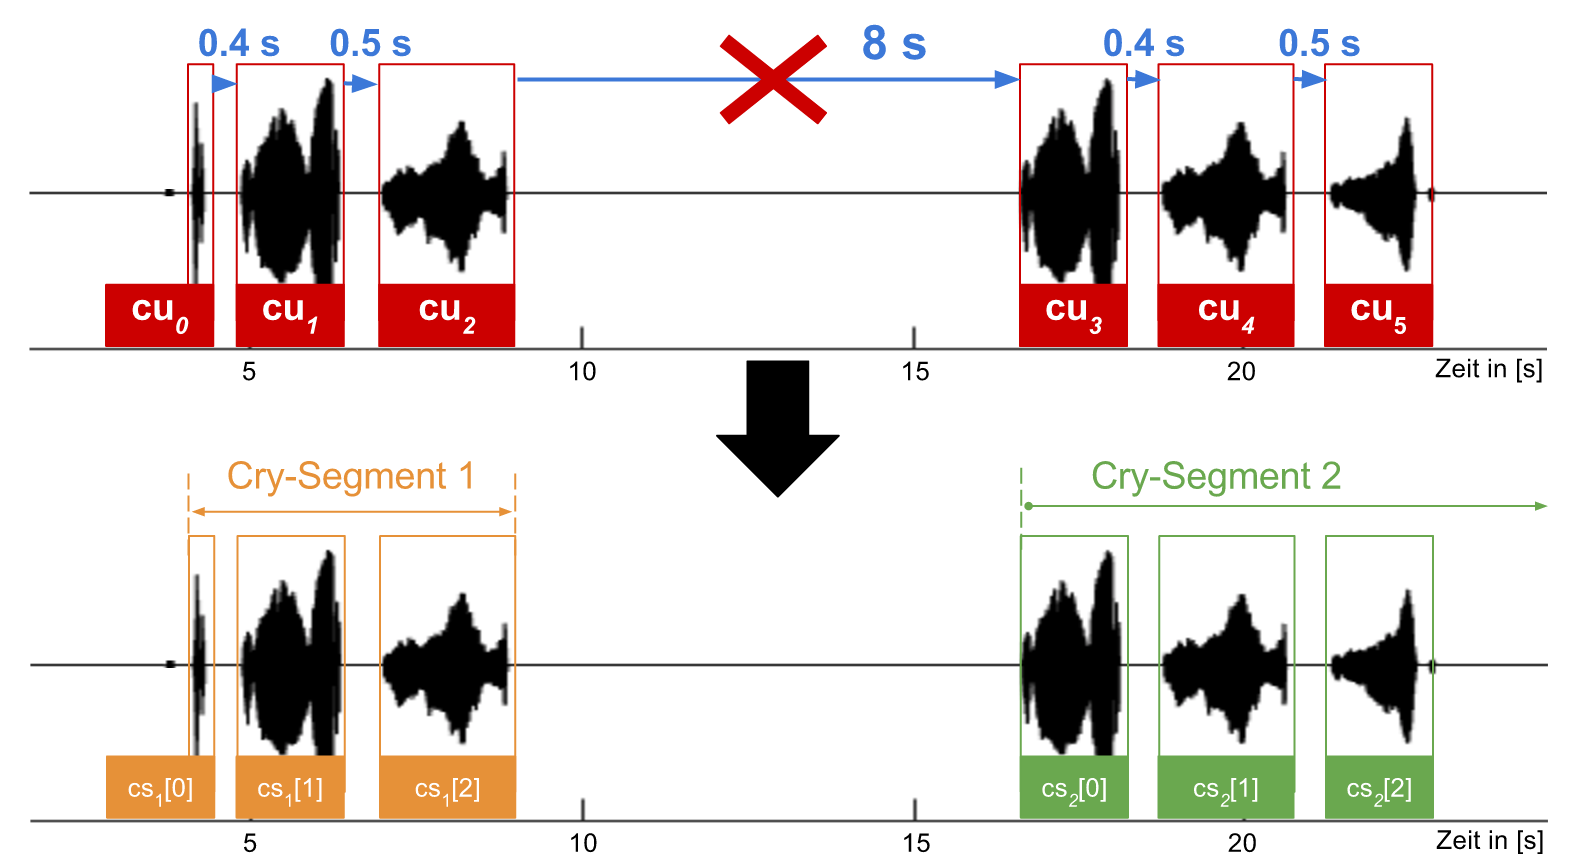
\includegraphics[width=1\textwidth]{bilder/segmentierung08.png}
	\caption[Beispiel für eine Segmentierung]{Beispiel für eine Segmentierung mit einem Grenzwert von $t_s = \SI{6}{\second}$}
	\label{img:segmenting06}
\end{figure}

Der Algorithmus eignet sich nicht für eine Online-Segmentierung, da das Ende eines Segmentes erst bei Beginn eines neuen Segmentes festgestellt wird, wobei beliebig viel Zeit zwischen den benachbarten Segmenten liegen kann. Wurde beispielsweise $t_{s} = \SI{1}{\minute}$ festgelegt, und die Pause zwischen zwei benachbarten Segmenten beträgt eine Stunde, so wäre das Ende des ersten Segmentes 59 Minuten zu spät festgestellt worden. Bei einer online durchgeführten Segmentierung empfiehlt es sich, die Dauer der Stille nach jeder neu erkannten Schreieinheit kontinuierlich zu messen und ein Segment sofort zu beenden, wenn ein Stillezeitraum den Grenzwert $t_s$ überschreitet.

\begin{algorithm}[h]
	\caption{Gruppierung von Schreieinheiten zu Schrei-Segmenten}
	\label{alg:crySegment}
	\begin{algorithmic}[1]
		\Function{segmentCryUnits}{$CU_{all}, t_{s}$}
		\State $ CS_{all} \gets [\;]$
		\State $ cs \gets [CU_{all}[0]]$
				\For{ $i = 1 , \ldots , length(CU_{all}) - 1$}
						\State $ cu_i \gets CU_{all}[i]$
						\State $cu_{i-1} \gets CU_{all}[i-1]$
						\If{d$(cu_{i-1},cu_i) < t_{seg-max}$}
								\State $cs \gets [cs_i , cu_i]$
						\Else
								\State $CS_{all} \gets [CS_{all}, cs]$
								\State $cs \gets [cu_i]$
						\EndIf
				\EndFor
		\Return $CS_{all}$
		
		\EndFunction
		
	\end{algorithmic}
\end{algorithm}


Das hier vorgestellte Segmentierungsverfahren wurde bewusst möglichst einfach gehalten, damit die Bedeutung des Parameters $t_{s}$ leicht ersichtlich ist und somit von der medizinischen Fachkraft selbständig festgelegt werden kann. Das Ende eines Segmentes ist weiterhin ein geeigneter Zeitpunkt, um die Parameter des Kompressors der Vorverarbeitungsstufe auf Basis des RMS-Wertes des Segmentes zu aktualisieren (siehe \autoref{sec:preprocessing}).


\section{Methoden zur Berechnung des Schmerz-Score für Segmente}
\label{sec:overviewPainRegression}

Das Ziel ist nun, nach dem Ende jeder Schmerzepisode einen Schmerz-Score für diese zu berechnen. Wie in Kapitel \ref{sec:medicalFoundations} erläutert wurde, ergibt sich ein Schmerz-Score aus der Summe der Scores, die für die einzelnen Schmerzindikatoren vergeben wurden. Auf Basis des akustischen Signals wird der Score des Schmerzindikators \emph{Weinen} berechnet. Betrachtet man allein diesen Schmerzindikator, so entspricht eine Schmerzepisode einem Schrei-Segment, wie im vergangenen Unterabschnitt argumentiert wurde.

Das nächste Teilproblem ist somit, \emph{Hypothesen} (auch: \emph{Modelle}, siehe \autoref{sec:learning}) zu finden, die für Schreisegmente Scores berechnen. Eine Hypothese ist abhängig von der jeweiligen Schmerz-Scale, da verschiedene Schmerz-Scales unterschiedliche Scorings definieren. Mathematisch formalisiert ist eine solche Hypothese $PC_{Scale}$ eine von der jeweiligen Schmerz-\emph{Scale} abhängige Funktion, die ein Schreisegment $cs \in CS$ auf einen von der Schmerz-Scale abhängigen \emph{Score} $s \in S_{Scale}$ abbildet, da heißt $PC_{Scale}: CS \mapsto S_{Scale}$. Die Bezeichnung der Funktion $PC$ verdeutlicht, dass die Hypothese zur Berechnung des Scores des Weinens (\textbf{P}ain-\textbf{C}ry) für die jeweilige Scale gedacht ist.

Angenommen, es soll die Schmerz-Scale \emph{NIPS} aus \autoref{tab:nips} zur Schmerzbewertung verwendet werden. In Bezug auf den Schmerzindikator \emph{Weinen} wird ein Score von 0 vergeben, wenn kein Weinen vorliegt, ein Score von 1, wenn das Weinen als \glqq mumbling\grqq{} (murmelnd) bewertet wird und ein Score von 2, wenn das Weinen als \glqq vigorous\grqq{} (energisch) bewertet wird. Formuliert als Modell $PC_{NIPS}:CS \mapsto \{0, 1 , 2\}$ ergibt sich:

\begin{equation}
PC_{NIPS}(cs) = \begin{cases}
 2 \quad ,\text{wenn } cs \text{ \glqq energisch ist\grqq } \\
 1 \quad ,\text{wenn } cs \text{ \glqq murmelnd ist\grqq } \\
 0 \quad ,\text{wenn } cs \text{ \glqq kein Weinen ist\grqq }
 \end{cases}	
\end{equation}

Das Problem ist offensichtlich: \glqq murmelnd\grqq{} und \glqq energisch\grqq{} sind subjektiv behaftete Begriffe und lassen sich nicht ohne weiteres aus den Eigenschaften eines Segmentes feststellen. Es muss somit für jede Schmerz-Scale eine Hypothese konstruiert werden, welches den Score für ein Schrei-Segment anhand \emph{objektiv messbarer Signaleigenschaften} berechnet. 

Die folgende Strategie wird vorgeschlagen, um für eine beliebige Schmerz-Scale eine solche Hypothese $PC_{Scale}$ zu gewinnen:

\begin{enumerate}
 \item Man erstellt eine Datenbank mit Audioaufnahmen mit dem Weinen von Babys. Jede Audioaufnahme wird so beschnitten, dass sie eine Scherzepisode / ein Schrei-Segment enthält.
 \item Man errechnet für jede Audioaufnahme \glqq so viele \emph{objektiv} messbare Eigenschaften wie möglich\grqq{}, wie zum Beispiel die insgesamt Segment-Länge, die durchschnittliche Länge der enthaltenen Schreieinheiten, durchschnittliche Tonhöhe usw.
 \item Man bittet medizinische Fachkräfte, für jede Aufnahme der Datenbank einen Score auf Basis der Kriterien der jeweiligen Schmerz-Scale zu vergeben, für die man eine Hypothese sucht. So erhält man einen gelabelte Trainingsdatensatz.
 \item Man trainiert einen \emph{Algorithmus zur ordinalen Regression} mit diesem Datensatz, um den Zusammenhang zwischen den in Schritt 2 objektiv gemessenen Eigenschaften der Schreisegmente und den in Schritt 3 vergebenen Scores herzustellen (siehe \autoref{sec:learning}). Es wird darauf hingewiesen, dass es sich hierbei \emph{nicht} um ein herkömmliches Regressionsproblem handelt, da die Schmerz-Scales Ordinalskalen, und keine kontinuierlichen Skalen definieren. In diesem Arbeitsschritt wird sich herausstellen, welche der Segment-Eigenschaften mit der Höhe des Scores korrelieren und zur Prognose sinnvoll sind. Das Ergebnis dieses Schrittes ist eine Hypothese $PC_{Scale}$.
\end{enumerate}

Eine Hypothese $PC_{Scale}$ kann daraufhin in dem automatisierten System eingesetzt werden, um für neue, bisher unbekannte Schrei-Segmente den Score für das Weinen zu prognostizieren. Der Vorteil dieser Vorgehensweise zur Erstellung der Hypothesen ist, dass das Problem der Übersetzung der objektiv messbaren Signaleigenschaften in die subjektiv behafteten Begriffe, die von den Schmerz-Scales verwendet werden, überbrückt wird, indem man die Regression direkt von den Signaleigenschaften auf den Score durchführt. Der Nachteil dieser Strategie ist, dass für jede Schmerz-Scale eine gesonderte Hypothese konstruiert werden muss, auch, wenn zwei Schmerz-Scales den selben subjektiv behafteten Begriff verwenden.

Dieser Vorschlag ist nur eines von mehreren denkbaren Vorgehen zur Gewinnung von Hypothesen für Schmerz-Scales. So könnte beispielsweise Anstatt der ordinalen Regression von den Segmenteigenschaften auf den Score eine Klassifizierung auf die subjektiv behafteten Begriffe durchgeführt werden, und diese daraufhin zur Berechnung des Scores zu verwenden. Es ist im zeitlichen Rahmen dieser Arbeit nicht möglich gewesen, selber Hypothesen für Schmerz-Scales nach dem vorgestellten Vorgehen zu erstellen. Die Akquise von Audioaufnahmen von Babys sowie die Schmerzbewertung dieser in Zusammenarbeit mit medizinischen Fachkräften erfordern nicht nur Zeit, sondern das Fachwissen über das Führen und die Auswerten von Interviews. 

In Hinblick auf die Schmerzbewertung im multimodalen Verbund ist es darüber hinaus notwendig, Hypothesen für die anderen Schmerzindikatoren zu erstellen. Der insgesamte Schmerz-Score einer Schmerzepisode ergibt sich daraufhin, indem alle Scores aufaddiert werden, die durch die Hypothesen der jeweiligen Schmerzindikatoren prognostiziert wurden. \autoref{eq:multimodal_pain_caluclation} verdeutlicht, nach welchem Muster eine solche Berechnung durchgeführt wird. $PF_{Scale}$ ist eine fiktive Funktion, die den Score für den Schmerzindikator \emph{Gesichtsausdruck} berechnet. Eine weitere Betrachtung dieser Berechnung liegt außerhalb des Rahmens dieser Arbeit. 

\begin{equation}
\text{Pain-Score}_{Scale} = PC_{Scale}(cs) + PF_{Scale}(face-Segment) + ...
\label{eq:multimodal_pain_caluclation}
\end{equation}


In den folgenden Teilabschnitte werden zwei Teilprobleme der automatisierten Schmerzbewertung des Weinens genauer beleuchtet. \autoref{sec:segmentFeatures} erläutert die Berechnung objektiv messbarer Eigenschaften für Schrei-Segmente, auf die sich die Hypothesen stützen können. In \autoref{sec:regressionTimeStuff} werden Möglichkeiten vorgestellt, um den Verlauf des Schmerzgrades innerhalb von Schrei-Segmenten auszuwerten.


%\vspace{5mm}

%\textbf{Strategie 1} \noindent\rule{0.83\linewidth}{0.3pt}\\
%... löst das Problem mit Hilfe von \emph{ordinaler Regression auf die Scores} (Siehe Abschnitt \ref{sec:learning}):
%\begin{enumerate}
 %\item Man erstellt eine Datenbank mit Aufnahmen von kindlichen Lautäußerungen, die man segmentiert.
 %\item Man errechnet \glqq so viele \emph{objektiv} messabare Eigenschaften wie möglich\grqq{} für jedes Segment, wie zum Beispiel die insgesamte Länge, die durchschnittliche Länge der enthaltenen Cry-Units, durchschnittliche Tonhöhe usw.
 %\item Man bittet medizinische Fachkräfte, für jedes Segment der Datenbank einen Score bezüglich der Schmerz-Scale zu vergeben, für den man den Predictor sucht. So erhält man einen gelabelte Trainingsdatensatz 
 %\item Man trainiert einen \emph{Algorithmus zur ordinalen Regression} mit diesem Datensatz, um den Zusammenhang zwischen den in Schritt 2 objektiv gemessenen Eigenschaften der Segmente und den in Schritt 3 vergebenen Scores herzustellen. Es wird darauf hingewiesen, dass es sich hierbei \emph{nicht} um ein herkömmliches Regressionsproblem handelt, da die Scales Ordinalskalen, und keine kontinuierlichen Skalen definieren. Man erhält somit einen Prediktor für jede Schmerz-Scale.
 %\item Möchte man für neue, unbekannte Segmente den Score bezüglich des Weinens prognostizieren, nutzt man den entsprechenden Regressor.
%\end{enumerate}
%\noindent\rule{\linewidth}{0.3pt}

%Das Vorteil dieses Vorgehens ist, dass das Problem der Übersetzung der objektiv messbaren Segmenteigenschaften in die subjektiv behafteten Begriffe, die in den Schmerz-Scales zum Scoring verwendet werden, überbrückt wird. Der Score wird direkt aus den objektiv messbaren Eigenschaften eines Segmentes berechnet. Der Nachteil ist, dass das Labeling zum Aufbau des Trainingsdatensatzes für jede Pain-Scale aufgebaut werden muss. Wird ein neue Pain-Scale eingeführt, muss der Prädiktor für diese Scale durch erneutes Labeln festgestellt werden. Ein weiterer Effekt der Abbildung des Problems als Regression ist, dass ein Regressor in einen kontinuierlichen Zahlenraum abbildet. Es sind also Regressionsergebnisse wie zum Beispiel $2.8$ denkbar. Diese \glqq bessere Auflösung\grqq{} kann als Vorteil betrachtet werden. Ist jedoch eine direkte Übersetzung der Pain Scale inklusive der ganzzahligen Punktzahlen gewünscht, so stellt sich die Frage, ob eine $2.8$ auf- oder abzurunden ist.

%\vspace{5mm}

%\textbf{Strategie 2} \noindent\rule{0.83\linewidth}{0.3pt} \\
%... löst das Problem mit Hilfe von Klassifizierung (Siehe Kapitel \ref{sec:classification}):
%\begin{enumerate}
%	\item und 2. entsprechen Strategie 1
%	\stepcounter{enumi}
%	\item Man sammelt alle subjektiven Begriffe, die in Pain Scales verwendet werden, wie zum Beispiel \glqq murmelnd\grqq , \glqq energisch\grqq , usw.
%	\item Man bittet medizinische Fachkräfte, jedes Segment der Datenbank mit denjenigen Begriffen zu labeln, die die jeweilige Person für zutreffend hält. 
%	\item  Man Verwendet einen \emph{Klassifizierungsgorithmus}, um einen Zusammenhang zwischen den in Schritt 2 festgestellten objektiv messbaren Eigenschaften der Segmente und den \emph{subjektiv behafteten Begriffen} zu finden. Man erhält somit einen Klassifikator für jeden Begriff, der binär in \emph{positive = zutreffend} und \emph{negative = nicht zutreffend} klassifiziert.
%	\item Möchte man für neue, unbekannte Segmente die Pain Score prognostizieren, so wird für jede mögliche Score der Pain Scale überprüft, ob für alle subjektiv beschreibenden Begriffe der entsprechende Klassifikator ein positive prognostiziert. Die Ableitung der Score ist somit ein weiters Klassifizierungsproblem, wobei eine Score einer Klasse entspricht und genau dann abgeleitet werden kann, wenn alle Vorraussetzungen für die Klasse erfüllt sind.
%\end{enumerate}
%\noindent\rule{\linewidth}{0.3pt}

%Der Vorteil dieser Methode ist, dass auch zum Zeitpunkt der Erstellung der Testdatenbank unbekannte Pain Scales zu einem späteren Zeitpunkt eingebunden werden können, insofern alle in dieser neuen Pain Scale verwendeten subjektiv behafteten Begriffe bereits gelabelt vorliegen, weil sie auch in anderen Pain Scales verwendet wurden. Das Vorgehen erlaubt somit eine gewissen Flexibilität bezüglich zukünftig entwickelter Pain Scales. Der Nachteil dieser Methode ist, dass durch die Umwandlung der eigentlich quantitativ geordenten Score einer Pain Scale in qualitative Klassen aus einem implizit als Regression zu betrachtenden Problem ein Klassifizierungsproblem macht. Dies wirft neue Fragen auf, wie zum Beispiel: Angenommen, bei einer fiktiven Pain Scale wird jede Score mit jeweils drei subjektiv behafteten Begriffen beschrieben, und bei der Klassifizierung eines Segmentes wird festgestellt, dass für jede Punktzahl genau zwei der drei Begriffe erfüllt werden. Welche Score wird dann prognostiziert? Ein anderes Beispiel wird am Beispiel der der NIPS-Score aus Tabelle \ref{tab:nips} verdeutlicht: Angenommen, ein Cry-Segment enthält hörbar \glqq starkes\grqq{} Schreien, es kann jedoch weder \glqq mumbling (murmelnd) \grqq{} noch \glqq vigorous (energisch)\grqq{} abgeleitet werden. Demzufolgen müsste dieses Segment eine Score von 0 Punkten erhalten, wobei ein Mensch in dieser Situation eventuell \glqq stark\grqq{} zu \glqq heftig\grqq{} uminterpretieren und 2 Punkte vergeben hätte. Strategie 1 ist weniger anfällig für dieses Problem.

%In jedem Fall werden medizinische Fachkräfte benötigt, um das Labeling der Cry-Segmente durchzuführen, was aus Zeitgründen im Rahmen dieser Arbeit nicht möglich ist. Die Aquise von Audioaufnahmen von Babys sowie das Labeling der Aufanhmen erfodern nicht nur Zeit, sondern das Fachwissen über das Führen und die Auswerten von Interviews.

\subsection{Extrahierung von Eigenschaften als Grundlage zur Schmerzbewertung}
\label{sec:segmentFeatures}

%Wie im vergangenen Abschnitt erläutert wurde, stützt sich eine Hypothese zur Berechnung eines Score für das Weinen auf objektiv messbare Eigenschaften der Schrei-Segmente. In diesem Kapitel werden Möglichkeiten zur Berechnung dieser Eigenschaften besprochen.

Varallyay \cite[S. 16 - 17]{cry_thesis} hat in seiner Dissertation vorgeschlagen, die Segment-Bezogenen Eigenschaften in drei Klassen einzuteilen: 1.) Eigenschaften des Zeitbereichs, 2.) Eigenschaften der Frequenzbereichs, und 3.) Melodie-bezogene Eigenschaften. Diese Kategorisierung wurde für die Einteilung der Eigenschaften übernommen. In den folgenden Unterabschnitten werden konkrete Eigenschaften definiert und Berechnungsvorschriften festgelegt. Die vorgestellten Eigenschaften orientieren sich an denen, die in \autoref{sec:acousticModel} im Zusammenhang mit der Schreiforschung vorgestellt wurden. Die Berechnungsvorschriften basieren auf den in dieser Arbeit eingeführten Datentypen \emph{Schrei-Segment} aus \autoref{eq:cry-segment} und \emph{Schreieinheit} aus \autoref{eq:cry-Unit}.

Das Ziel dieses Abschnittes ist vor Allem, Möglichkeiten der Analyse der Schrei-Segmente zu demonstrieren. Es handelt sich hierbei nicht um eine vollständige Formalisierung aller in der Literatur genannten Eigenschaften, die zur Prognose von Emotionen, Krankheiten oder Schmerzstärken verwendet wurden. Weiterhin ist es in dieser Arbeit nicht möglich, festzustellen, welche der definierten Eigenschaften sinnvoll für die Prognose von Schmerz-Scores sind, da dies ohne die Erstellung von Hypothesen nicht möglich ist.

%Im vergangenen Kapitel wurde erläutert, dass die Basis für die Ableitung einer Pain Score für ein Segment die Extraktion von \glqq so vielen Features wie möglich\grqq{} ist. In diesem Kapitel wird präzisiert, welche Features gemeint sind.  Varallyay \cite[S. 16 - 17]{cry_thesis} schlug vor, drei Kategorien an Features zu betrachten: 1.) Features des Zeitbereichs, 2.) Features der Frequenzbereichs, und 3.) Melodie-bezogene Attribute. Diese Kategorisierung wurde für diese Arbeit übernommen.

%In Kapitel \ref{sec:acousticModel} wurde beschrieben, welche Features in der medizinischen Schreiforschung typischerweise extrahiert wurden. In Kapitel \ref{sec:cryDiscussion} wurde diskutiert, dass 1.) nicht bewiesen ist, welche Features die \glqq wichtigsten\grqq{} sind und 2.) keine Einigung darüber herrscht, wie genau bestimmte Features zu berechnen sind. Basierend auf den in diesem Kapitel vorgestellten Features werden in diesem Kapitel konkrete Berechnungsvorschriften definiert. Welche von diesen Features tatsächlich im Zusammenhang mit Schmerz stehen, lässt sich erst in der anschließenden Nutzung der Features zur Regression oder Klassifizierung der Pain Scales feststellen, welche jedoch im Rahmen dieser Arbeit nicht durchgeführt werden kann.

\subsubsection{Eigenschaften des Zeitbereiches}

Mit Features des Zeitbereiches sind solche gemeint, die sich allein aus Kenntnis der Start- und Endzeitpunkte der im Segment enthaltenen Schreieinheiten sowie deren Zeitbereiche gewinnen lassen, wie beispielsweise die durchschnittliche Länge der Schreieinheiten oder die durchschnittliche Energie der Schreieinheiten.\cite[S. 16 - 17]{cry_thesis} In diesem Kapitel gilt die Konvention, dass eine Schrei-Segment $cs$ insgesamt $N$ Schreieinheiten enthält, der Indexbereich wird mit $0 \ldots N-1$ definiert.

\begin{description}
\item[Segment-Length: ] Die zeitliche Länge eines Segmentes wird nach \autoref{eq:segment_length} berechnet:
\begin{equation}
\text{S-Length}(cs) = cs[N-1].end - cs[0].start
\label{eq:segment_length}
\end{equation}

\item[Density: ] Der Relativer Anteil der Länge der Schreieinheiten an der Länge des Segmentes wird nach \autoref{eq:segment_density} berechnet. Die Länge einer Schreieinheit wurde in \autoref{eq:cry-Lambda} definiert.
\begin{equation}
\text{Density}(cs) = \frac{\sum_{i = 0}^{N-1} \lambda(cs[i])}{\text{Segment-Length}(cs)}
\label{eq:segment_density}
\end{equation}

\item[Tempo:] Diese Eigenschaft beschreibt das Verhältnis zwischen der Anzahl an Schreieinheiten und der Dauer des Segmentes. Die Eigenschaft ähnelt dem von LaGasse et al. \cite[S. 85]{parentalPerception} als \emph{Utterances} bezeichneten Feature.

\begin{equation}
\text{Tempo}(cs) =  \frac{N}{\text{S-Length}(cs)}
\end{equation}

\item[Statistics of Cry-Units:] Es können statistische Kennwerte bezüglich der \emph{Längen aller Schreieinheiten} eines Schrei-Segmentes berechnet werden. \autoref{eq:featuresOfCryUnits} zeigt, wie der Durchschnitt, Median, Minimum, Maximum sowie die Standardabweichung der Länge der Schreieinheiten berechnet werden. Diese Liste an statistischen Kenngrößen lässt sich beliebig erweitern, beispielsweise durch die Bestimmung von Quartilen. Das $\text{mean}_{cu}(cs)$-Feature wurde von LaGasse et al. \cite[S. 85]{parentalPerception} und in weiteren Veröffentlichung als \emph{Mean Duration} bezeichnet. Diese Kenngrößen wurden unter anderem von Zeskind et al. \cite{rythmic} bei der Untersuchung des Weinens Neugeborener berechnet.

\begin{equation}
\begin{gathered}
\text{mean}_{cu}(cs) = \meani_{i = 0 \ldots N-1}\{\lambda(cs[i])\} \\
\text{median}_{cu}(cs) = \mediani_{i = 0 \ldots N-1}\{\lambda(cs[i])\} \\
\text{min}_{cu}(cs) = \mini_{i = 0 \ldots N-1}\{\lambda(cs[i])\} \\
\text{max}_{cu}(cs) = \maxi_{i = 0 \ldots N-1}\{\lambda(cs[i])\} \\
\sigma_{cu}(cs) =  \sigma_{i = 0 \ldots N-1}\{\lambda(cs[i])\} 
\end{gathered}
\label{eq:featuresOfCryUnits}
\end{equation}

\item[Statistics of Bursts:]\footnote{Erläuterung zum Begriff \emph{Burst} in \autoref{sec:acousticModel}} Die in \autoref{eq:featuresOfCryUnits} definierten statistischen Kennwerte können ebenso in Bezug auf die \emph{Längen aller Bursts} eines Segmentes errechnet werden, in dem in jeder Gleichung $\lambda(cs[i])$ ersetzt wird durch $cs[i].start - cs[i-1].start$. Die Indexierung muss auf $i = 1 ,\ldots, N-1$ begrenzt werden. In \autoref{eq:featuresOfBursts} wird nur die Berechnung der durchschnittlichen Länge aller Bursts gezeigt, da die Berechnungsvorschriften weiterer statistischer Kennwerte nach dem Prinzip aus \autoref{eq:featuresOfCryUnits} ersichtlich sind. Diese Kenngrößen wurden ebenfalls von Zeskind et al. \cite{rythmic} in Untersuchungen verwendet.

\begin{equation}
\begin{gathered}
\text{mean}_{burst}(cs) = \meani_{i = 1 \ldots N-1}\{cs[i].start - cs[i-1].start\} \\
\ldots
\end{gathered}
\label{eq:featuresOfBursts}
\end{equation}

\item[Statistics of Pauses:] Nach dem selben Muster werden statistische Kennwerte bezüglich der  \emph{Längen aller Pausen} eines Segmentes ermittelt. Eine Pause entspricht in diesem Zusammenhang der Distanz zwischen zwei auf einander folgenden Schreieinheiten nach \autoref{eq:cry-distance}.

\begin{equation}
\begin{gathered}
\text{mean}_{pause}(cs) = \meani_{i = 1 \ldots N-1}\{d(cs[i-1],cs[i])\} \\
\ldots
\end{gathered}
\label{eq:featuresOfPauses}
\end{equation}

\item[Statistics of Energies:] Zunächst wird die Liste aller in den Schreieinheiten eines Segmentes enthaltenen Signalfenster definiert nach \autoref{eq:windowsOfSegment}. Eine Schreieinheit enthält die Signalfenster $cu.windows = x_0[\;],\ldots,x_n[\;]$

\begin{equation}
x_{seg}[\; ] = cs[0].windows[0] \;  , \; \ldots \; , \; cs[N-1].windows[n] 
\label{eq:windowsOfSegment}
\end{equation}

Die Liste $x_{seg}[\; ]$ enthält $R$ Signalfenster, die Indexierung wird definiert mit $0, \ldots, R-1$.  \autoref{eq:energyStats} definiert die Berechnung statistischer Kennwerte bezüglich der \glqq Lautstärke Segmentes\grqq. Der MSV-Wert als Maß des durchschnittlichen Energiegehaltes wurde in \autoref{eq:msv} definiert.

\begin{equation}
\begin{gathered}
\text{mean}_{msv}(cs) = \meani_{i = 0 \ldots R-1}\{MSV(x_{seg}[i])\} \\
\ldots
\end{gathered}
\label{eq:energyStats}
\end{equation}

\end{description}

Es wird angemerkt, dass in der Schreiforschung zeitliche Eigenschaften im geringeren Maße in Betracht gezogen wurden als Features des Frequenz-Bereiches. Die einzigen zeitliche Features, die zum Beispiel von Wasz-Hockert et al. \cite{25years}, Fuller \cite{threeCryTypes} und LaGasse et al. \cite{parentalPerception} berechneten wurden, sind \emph{die durchschnittliche Länge der Schreieinheiten} sowie die \emph{Latenz zwischen Reiz und erster Schreieinheit der Schmerzantwort}. Die durchschnittliche Länge der Schreieinheiten wurde in \autoref{eq:featuresOfCryUnits} definiert, die Latenz kann jedoch nur auf Basis des Audiosignals nicht festgestellt werden. Die anschließende Nutzung der Features zur Erstellung der Hypothesen wird Auskunft darüber geben, welchen Beitrag Eigenschaften des Zeitbereichs zur Schmerzdiagnose leisten können.

\subsubsection{Eigenschaften des Frequenzbereiches und der Melodie}

Als Grundlage zur Definition von Segmenteigenschaften des Frequenzbereiches werden alle Signalfenster der Schreieinheiten eines Segmentes in den Frequenzbereich transformiert und in der Liste $X_{seg}[\;]$ nach \ref{eq:specOfSegment} gesammelt. Dies entspricht der Kurzzeit-Fourier-Transformation aller Schreieinheiten des Segmentes (siehe \autoref{sec:stft}). Die Indexierung von $X_{seg}[\;]$ läuft, wie bei $x_{seg}$, von $0 , \ldots , R-1$. Analog dazu wird die Liste aller Cepstren der Schreieinheiten eines Segmentes $c_{seg}[\;]$ definiert. 

\begin{equation}
X_{seg}[\; ] = \Big[ |DFT\{x_{seg}[0] \cdot w[\;]\}| \; , \ldots , \; |DFT\{x_{seg}[R-1] \cdot w[\;]\}| \Big]
\label{eq:specOfSegment}
\end{equation}


Die folgenden Eigenschaften des Frequenzbereiches lassen sich mit den in dieser Arbeit vorgestellten Methoden berechnen:

\begin{description}
\item[Ratio2:] Diese Eigenschaft wurde von Fuller \cite{threeCryTypes} definiert und beschreibt die Spannung des Vokaltraktes als Verhältnis der Energien oberhalb von \SI{2000}{\hertz} zu den Energien unterhalb \SI{2000}{\hertz}. Wie bei den Eigenschaften des Zeitbereiches können verschiedene statistische Kennwerte bezüglich dieser Eigenschaft berechnet werden. \autoref{eq:ratio2} zeigt die Berechnung des Durchschnitts.

\begin{equation}
\begin{gathered}
\text{mean}_{Ratio2}(cs) = \meani_{i=0\ldots R-1} \Big\{ \frac{\sum_{k=0}^{\SI{2000}{\hertz}} X_{sec}[i][k]^2}{\sum_{j=\SI{2000}{\hertz}}^{f_{s}} X_{sec}[i][j]^2} \Big\} \\
\ldots
\end{gathered}
\label{eq:ratio2}
\end{equation}


\item[Clarity: ] Wie in Kapitel \ref{sec:vad_ceps_features} erläutert wurde, deutet eine klar ausgebildete Spitze im oberen Cepstrum-Bereich auf ein stimmhaftes Signal hin. Ein hoher Anteil hoher Cepstrum-Peaks lässt somit auf vermehrt phonierte Laute schließen, geringere Cepstrum-Peaks auf dysphoniertere Laute (Siehe Kapitel \ref{sec:acousticModel}). Der Durchschnittswert dieser Eigenschaft ist ein Maß für den relativen Anteil dysphonierter Laute, die Standardabweichung ähnelt dem in Kapitel \ref{sec:acousticModel} vorgestellten \emph{Cry-Mode Changes}-Feature.

\begin{equation}
\begin{gathered}
\text{mean}_{Clarity}(cs) = \meani_{i=0\ldots R-1} \Big\{ Ceps_{mag}(c_{seg}[i])  \Big\} \\
\ldots
\end{gathered}
\end{equation}
	
	
\end{description}

Alle weiteren Eigenschaften, die in Kapitel \ref{sec:acousticModel} vorgestellt wurden und sich auf den Frequenzbereich oder den Melodieverlauf der Schreieinheiten beziehen, lassen sich nicht mit den in dieser Arbeit vorgestellten Methoden umsetzen, da diese Eigenschaften auf der Berechnung der Formanten und der Grundtonhöhe basieren. Die Berechnung der Formanten und der Grundtonhöhe ist ein Bereich, der seit vielen Jahren erforscht wird und für den eine Vielzahl robuster Algorithmen entworfen wurden. Die Form, die diese Eigenschaften annehmen würden, sollte aus den bisher vorgestellten Features ersichtlich sein. 

%Bei allen vorgestellten Eigenschaften handelt es sich, nach dem Vorbild der in Kapitel \ref{sec:acousticModel} vorgestellten Methoden der klassischen Schreiforschung, um solche, bei denen die Reihenfolge der Cry-Units nicht mit in Betracht gezogen wird. Angenommen, ein Segment besteht aus $n$ Cry-Units, wobei genau eine hälfte der  Cry-Units kurz und die andere hälfte der Cry-Units lang ist. Das $\text{stats}_{cu}(cs)$-Feature wird bezüglich des Durchschnittes, Minimum, Maximum etc. die selben Werte berechnen, unabhängig davon, ob sich die kurzen Cry-Units allesamt am Beginn des Segmentes, am Ende des Segmentes oder mit den langen Cry-Units durchmischt befinden. Bei der anschließenden Nutzung der Features zu Regression/Klassifizierung wird sich zeigen, wie sehr sich diese Features zur Ableitung von Pain-Scores eignen. Stellt sich heraus, dass sich die Features nicht eignen, ist es eventuell notwendig, neue Features zu definieren, die die Position der Cry-Units mit in Betracht ziehen.

\subsection{Betrachtung des Schmerzverlaufs innerhalb von Segmenten}
\label{sec:regressionTimeStuff}

Aus \autoref{sec:segmenting} ging hervor, dass nach dem vorgestellten Konzept die Schmerzbewertung des Weinens bei Beendigung eines Schrei-Segmentes vorgenommen wird. Dieses Vorgehen hat die folgenden Nachteile:
\begin{enumerate}
\item Es ist denkbar, dass die Bewertung der Schmerzstärke erst zu Ende einer Schmerzepisode zu spät für einige Anwendungsfälle ist, insbesondere bei der Schmerzdiagnose während schmerzversachenden Eingriffen. Es ist daher wünschenswert, ein Methode zur Berechnung von \glqq Zwischenergebnissen\grqq{} anzubieten, noch bevor ein offenes Segment abgeschlossen wurde.
\item Falls der Schmerz innerhalb eines Segmentes stark ab- oder zunimmt, ist dieser Verlauf nicht erkennbar, da nach der vorgestellten Methode jediglich der \glqq durchschnittliche Schmerz\grqq{} des Segmentes prognostiziert wird.
\end{enumerate}

Das vorgestellte Segmentierungs- und Bewertungsprinzip wird daher erweitert durch eine \emph{Aktualisierungsfrequenz} $[f_{act}]$ und einen \emph{Beobachtungszeitraum} $[t_{obs}]$ erweitert, welche in den folgenden Unterabschnitten näher erläutert werden.

\subsubsection{Aktualisierungsfrequenz}
\label{sec:actualization}

 Die grundlegende Idee der Aktualisierungsfrequenz ist, innerhalb eines momentan offenen Schreisegments in regelmäßigen Abständen den Schmerzgrad auf Grundlage der bisherigen Segmenteigenschaften festzustellen, um häufiger Zwischenergebnisse bezüglich des Schmerzgrades zu erhalten. Die höchstmögliche, sinnvolle Aktualisierungshäufigkeit ist die Berechnung eines Schmerz-Scores nach jeder dem Segment neu hinzugefügten Schreieinheit. Die geringst mögliche Aktualisierungshäufigkeit ist, gar keine Aktualisierungen durchzuführen und den Schmerz-Score erst bei Beendigung des jeweiligen Schrei-Segmentes zu berechnen.
 
Es wird vorgeschlagen, $f_{act}$ als Frequenz festzulegen. Eine Aktualisierungsfrequenz von beispielsweise $f_{act} = \SI{1/10}{\second}$ bedeutet, dass alle 10 Sekunden ein Schmerz-Score für ein Segment berechnet wird. Die Beendigung eines Segmentes soll in jedem Fall eine Berechnung eines Schmerz-Score auslösen und einen \glqq erzwungenen Aktualisierungszeitpunkt\grqq{} darstellen. Die folgenden Möglichkeiten zur Bestimmung von sinnvollen Frequenzwerten $f_{act}$ werden vorgeschlagen:
 
 \begin{itemize}
 \item Die Festlegung einer globalen Aktualisierungsfrequenz unabhängig von der verwendeten Schmerz-Scale. Ein solcher Wert müsste in Absprache mit medizinischen Fachkräften eruiert werden.
 \item Es wird der medizinischen Fachkraft überlassen, die das System bedient, eine Aktualisierungsfrequenz festzulegen. So kann die jeweilige Person selber bestimmen, wie häufig sie eine Aktualisierung der Schmerzbewertung wünscht.
 \item Die feste Bindung der Aktualisierungsfrequenz an die verwendete Schmerz-Scale. Die CRIES-Scale ist beispielsweise für das post-operative Monitoring gedacht und benötigt somit möglicherweise weniger häufige Aktualisierungen als der DAN, welcher zur Schmerzdiagnostik während einer Operation eingesetzt wird (siehe \autoref{tab:painscores}).
 \end{itemize}
 
Unabhängig von der verwendeten Variante kann es durch den Einsatz einer Aktualisierungsfrequenz passieren, dass eine Aktualisierung in einem offenen Segment durchgeführt wird, während gerade eine neue Schreieinheit detektiert wird und noch nicht abgeschlossen wurde. Es wurde die Entscheidung getroffen, eine solche unabgeschlossene Schreieinheit \emph{nicht} mit in die Schmerzbewertung einzubeziehen. Der Hintergrund für diese Entscheidung ist, dass bestimmte Hypothesen ansonsten fehlerhafte Prognose treffen können. Würde beispielsweise eine Hypothese den Schmerzgrad anhand der geringste Länge einer Schreieinheit im Segment prognostizieren, würde eine unvollständige Schreieinheit das Ergebnis verfälschen.
 
%Die Berechnung des Scores mit der Hypothese $PC_{Scale}$ wird bei eine Aktualisierung für ein \emph{Subsegment} $cs_{sub}$ durchgeführt, welches alle Schreieinheiten des noch gesamten, offenen Segmentes $cs$ übernimmt, die zum Aktualisierungszeitpunkt $t$ vollständig begonnen und beendet wurden. Der Endzeitpunkt des Subsegmentes wird, wie bei herkömmlichen Segmenten, auf den Endzeitpunkt der letzten vollständigen Schreieinheit im Subsegment gesetzt.
  
 \subsubsection{Beobachtungszeitraum}
 
Angenommen, einem Baby wird akuter Schmerz zugefügt, indem es mit einer Nadel in den Fuß gestochen wird. Das Baby empfindet kurz nach dem Nadelstich einen starken Schmerz, welcher nach dem Verstreichen einiger Zeit abnimmt und schlussendlich vollständig verschwindet. Der anfängliche, starke Schmerz würde sich durch lange Schreieinheiten mit hoher Tonhöhe zeigen, die geringere Schmerz gegen Ende durch tendenziell kürzere Schreieinheiten mit niedrigerer Tonhöhe.\cite{acutePainResponse} Das automatisierte Schmerzbewertungsystem würde für diese Schmerzepisode ein Schreisegment eröffnen und, je nach Aktualisierungsintervall, in regelmäßigen Abständen so wie bei Beendigung des Schreisegmentes die Schmerz-Scores auf Basis des Weinens prognostizieren. Angenommen, die Hypothese schließt einen hohen Schmerz vor allem aus dem Vorhandensein von Schreieinheiten mit hoher Tonhöhe. In diesem Fall würde zu jeder Aktualisierung ein hoher Schmerzgrad festgestellt werden, da die ersten, langen Schreieinheiten bei jeder Schmerzbewertung mit einbezogen wrden. Die Abnahme der Schmerzstärke gegen Ende wäre so bei keiner Aktualisierung sichtbar. Es kann argumentiert werden, dass in diesem Fall die Hypothese das Problem darstellt und optimiert werden müsste. Eine weitere Lösungsmöglichkeit, die in diesem Unterabschnitt vorgestellt wird, ist die Verwendung eines \emph{Beobachtungszeitraums} $t_{obs}$

Dieser Beobachtungszeitraum $t_{obs}$ definiert, welcher Zeitraum als Grundlage für die Schmerzbewertung innerhalb eines Segmentes mit einbezogen wird. Ein Wert von $t_{obs} = \SI{1}{\minute}$ würde beispielsweise bedeuten, dass  zu einem beliebigen Aktualisierungszeitpunkt nur diejenigen Schreigeräusche mit einbezogen werden, die innerhalb der letzten Minute aufgenommen wurden, auch, wenn das Schreisegment eigentlich bereits länger andauert. In Bezug auf das eben genannte Beispiel würden nach einer gewissen Zeit die ersten, höheren Schreisegmente nicht mehr in die Schmerzbewertung mit einfließen und so die Abnahme des Schmerzes sichtbar werden.

Es werden verschiedene Varianten zur Festlegung eines zeitlichen Wertes für $t_{obs}$ vorgestellt:
\begin{itemize}
\item Festlegung eines globalen oder eines von der medizinischen Fachkraft frei wählbaren Wertes, so wie bei der Aktualisierungsfrequenz $t_{act}$.
\item Die feste Bindung des Aktualisierungsintervalls an die jeweilige Schmerz-Scale. Hier könnten die Beobachtungszeiträume übernommen werden, die in den Anwendungsvorschriften die jeweilige Schmerz-Scale empfohlen werden (siehe Tabelle \ref{tab:painscores}). Es müsst wiederum in Zusammenarbeit mit medizinischen Fachkräften eruiert werden, ob diese, für die manuelle Schmerzdiagnostik vorgesehenen Werte auch für ein automatisiertes System Sinn machen.
\item Eine weitere Variante ist, $t_{obs}$ an den Wert von $f_{act}$ zu binden, womit einer der Werte den anderen bedingt. Ein Verhältnis von $t_{obs} = k \cdot 1/f_{act}$ würde beispeilsweise mit $k=1$ nicht-überlappende Beobachtungszeiträume und  mit $k=2$ überlappende Beobachtungszeiträume erzeugen.
\end{itemize}

Die Verwendung einer Aktualisierungsfrequenz und eines Beobachtungszeitraumes führen dazu, dass die Schmerzbewertung anstatt für ein gesamtes Segment $cs$ für ein \emph{Subsegment} $cs_{sub}$ durchgeführt wird. Ein solches Subsegment $cs_{sub}$ wird zu einem Aktualisierungszeitpunkt $t$ gebildet und übernimmt alle \emph{vollständigen} Schreieinheiten des Segments $cs$ innerhalb des Zeitraumes $t - t_{obs}$ bis $t$. Mit \emph{vollständigen} Schreieinheiten sind solche gemeint, die innerhalb dieses Zeitraumes komplett begonnen und beendet wurden. Anfangs- und Endzeitpunkt eines Subsegmentes werden, wie bei herkömmlichen Schreisegmenten, definiert durch den Anfangszeitpunkt der ersten Schreieinheit und dem Endzeitpunkt der letzten Schreieinheit des Subsegmentes. 

\vspace{5mm}

\section{Beispiel für die automatisierte Schmerzbewertung}

Die in diesem Kapitel vorgestellten Methoden zur Schmerzbewertung anhand akustischer Signale werden an einem Beispiel verdeutlicht. Tabelle \ref{tab:fiction_scale} zeigt die Schmerzbewertung des Weinens der \glqq Neonatal Infant Pain Scale\grqq{}.

\begin{table}[h]
\centering
\caption[Bewertung des Weinens bei der NIPS]{Bewertung des Weinens bei der NIPS \cite{nips}}
\label{tab:fiction_scale}
\begin{tabular}{@{}llll@{}}
\toprule
              & 0 Punkte    & 1 Punkt         & 2 Punkte       \\ \midrule
Fiction Scale & absent & mumbling & vigorous \\ \bottomrule
\end{tabular}
\end{table}

Es wird angenommen, dass für diese Schmerz-Scale mit Hilfe der in \autoref{sec:overviewPainRegression} beschriebenen Strategie eine Hypothese $PC_{NIPS}: CS \mapsto \{0,1,2\}$ ermittelt wurde, definiert \autoref{eq:ps_fiction}. Diese Hypothese ist fiktiv und wird nur zur Verdeutlichung des Beispiels verwendet.

\begin{equation}
PC_{NIPS}(cs) = \begin{cases}
 0 \quad ,  \text{wenn } mean_{cu}(cs) < \SI{0.3}{\second} \\
 1 \quad ,  \text{wenn } mean_{cu}(cs) < \SI{1}{\second} \\
 2 \quad ,  \text{wenn } mean_{cu}(cs) \geq \SI{1}{\second}
 \end{cases}	
 \label{eq:ps_fiction}
\end{equation}

\begin{figure}[h]
	\centering
	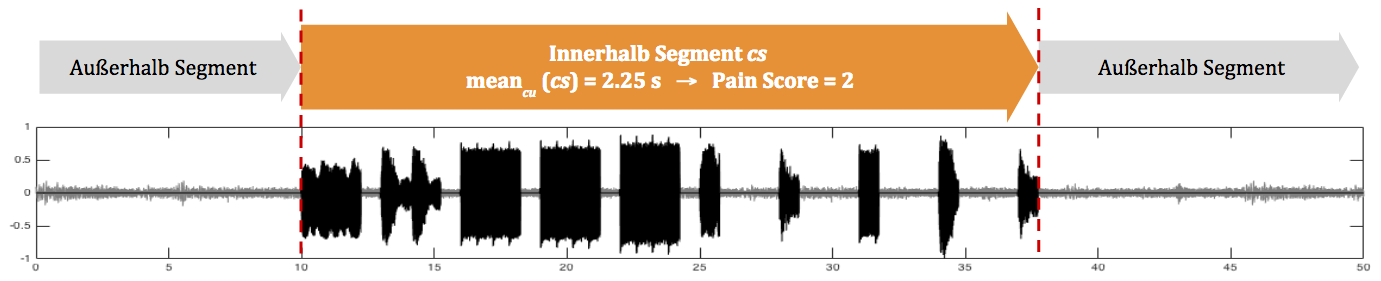
\includegraphics[width=1\textwidth]{bilder/regression_score_example04.png}
	\caption{Beispiel für die Ableitung von Pain Scores für ein Signal nach einer fiktiven Pain Scale ohne Beobachtungszeitraum oder Aktualisierungsintervall}
	\label{img:regression_score_example01}
\end{figure}


\autoref{img:regression_score_example01} zeigt ein Beispielsignal, für das Pain Scores nach dieser Pain Scale abgeleitet werden. In dem Signal werden die stimmhaften Signalbereiche schwarz und das Hintergrundrauschen grau dargestellt. Es sind insgesamt 10 Cry-Units zu erkennen. Die ersten fünf Cry-Units haben jeweils eine Länge von \SI{2.25}{\second}, die letzten fünf Cry-Units eine jeweilige Länge von \SI{0.75}{\second}. Das Signal wurde nach der in Kapitel \ref{sec:segmenting} beschriebenen Methode segmentiert mit $t_s = \SI{5}{\second}$ und so alle 10 Cry-Units zu einem Segment zusammengefasst. Das Segment erstreckt sich von Sekunde $10$ bis Sekunde $37.5$. Für das Segment wurde eine durchschnittliche Länge der Cry-Units von $mean_{cu}(cs) = \SI{1.5}{\second}$ gemessen und dem zufolge eine Pain Score von 2 abgeleitet. In diesem Fall wurde ohne Beobachtungs- und Aktualisierungsintervall gearbeitet. Wäre die Analyse also kontinuierlich vorgenommen worden, so wäre nach Feststellung der ersten Cry-Unit das Segment eröffnet, nach Überschreitung der maximal zulässigen Stille von $t_s = \SI{5}{\second}$ nach der 10. Cry-Unit das Segment geschlossen, und daraufhin $PS_{Fiction}(cs) = 2$ berechnet worden.

\begin{figure}[h]
	\centering
	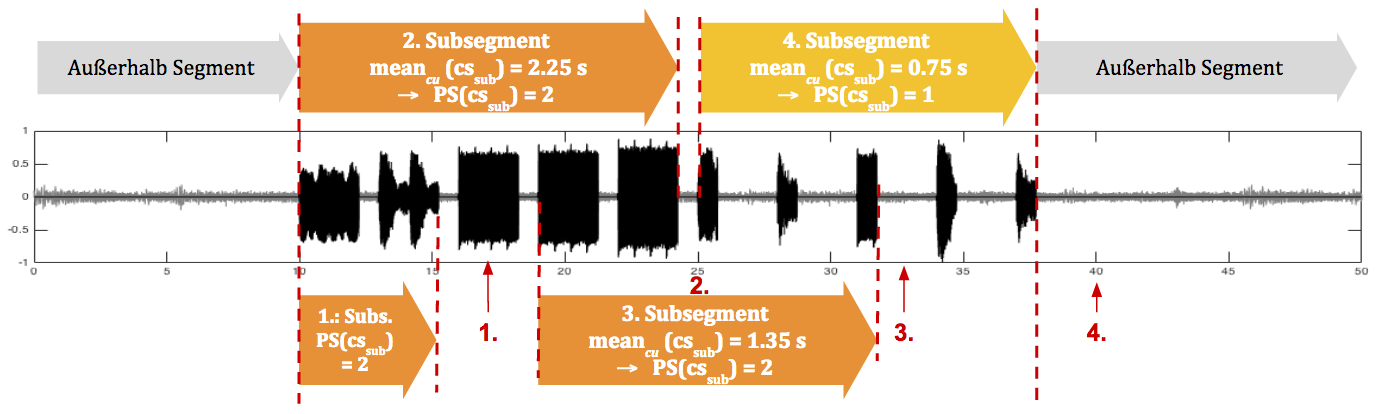
\includegraphics[width=1\textwidth]{bilder/regression_score_example05.png}
	\caption{Beispiel für die Ableitung von Pain Scores für ein Signal nach einer fiktiven Pain Scale mit $t_{act} = \SI{7.5}{\second}$ und $t_{obs} = \SI{15}{\second}$}
	\label{img:regression_score_example02}
\end{figure}

Abbildung \ref{img:regression_score_example03} zeigt die Ableitung der Schmerz Scores, wenn zusätzlich ein Aktualisierungsintervall von \SI{7.5}{\second} und ein Beobachtungszeitraum von \SI{15}{\second} gewählt wird. Nach dem das Segment durch die Cry-Unit an Sekunde 10 eröffnet wurde, werden Aktualisierungen zu den Zeitpunkten $t = \SI{17.5}{\second}, \SI{25}{\second}, \SI{32.5}{\second}$ und \SI{40}{\second} durchgeführt, verdeutlicht durch die kleinen, roten Pfeile in der Abbildung. Wie zu sehen ist, wird bei jeder Aktualisierung innerhalb des Beobachtungszeitraumes ein Subsegment gebildet, für das Subsegment die Features errechnet und die Pain Score abgeleitet. Der Anfangszeitpunkt jedes Subsegmentes ist der Anfang der erste Cry-Unit innerhalb des jeweiligen Beobachtungszeitraums, und das Ende des Subsegmentes das Ende letzten Cry-Unit im jeweiligen Beobachtungszeitraum. Beispielsweise erstreckt sich das bei der 3. Aktualisierung der Beobachtungszeitraum von $17.5 - \SI{32.5}{\second}$, das Subsegment jedoch von $19 - \SI{32}{\second}$ aufgrund der Lage der Cry-Units. Durch die Verwendung des Beobachtungs- und Aktualisierungsintervalls wird erkennbar, dass in diesem Beispiel der Schmerzgrad innerhalb des Segmentes nach hinten hin abnimmt.


